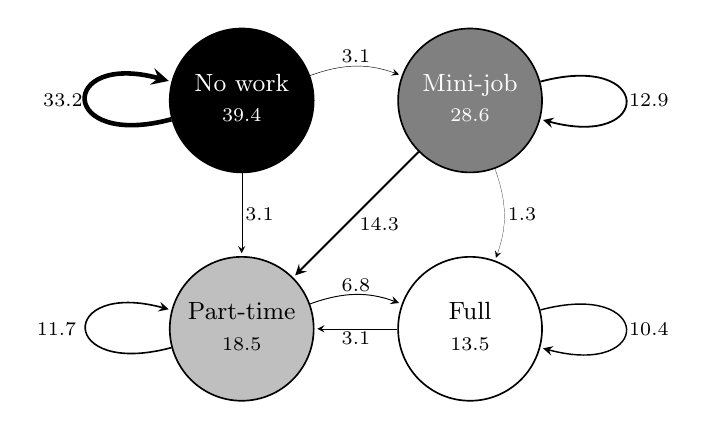
\begin{tikzpicture}[->,>=stealth,shorten >=1pt,auto,node distance=2.9cm, semithick] \tikzstyle{state}=[circle,fill=gray,draw=black,text=white]\node[state, fill=black,     minimum size=52pt, inner sep = -3pt]              (1)               {\small \begin{tabular}{c} No work  \\ {\scriptsize39.4}\end{tabular}}; \node[state, fill=gray,      minimum size=52pt, inner sep = -3pt]              (2) [right of=1]  {\small \begin{tabular}{c} Mini-job \\ {\scriptsize28.6}\end{tabular}}; \node[state, fill=lightgray, text=black, minimum size=52pt, inner sep = -3pt]  (3) [below of=1]  {\small \begin{tabular}{c} Part-time\\ {\scriptsize18.5}\end{tabular}}; \node[state, fill=white,     text=black,  minimum size=52pt, inner sep = -3pt] (4) [right of=3]  {\small \begin{tabular}{c} Full     \\ {\scriptsize13.5}\end{tabular}};\path(1) edge[line width=1.66pt,loop left,outer sep=-2pt] node {\scriptsize 33.2} (1)(1) edge[line width=0.16pt,bend left=20,outer sep=-2pt] node {\scriptsize 3.1} (2)(1) edge[line width=0.15pt,outer sep=-2pt] node {\scriptsize 3.1} (3)(2) edge[line width=0.65pt,loop right=20,outer sep=-2pt] node {\scriptsize 12.9} (2)(2) edge[line width=0.72pt,outer sep=-2pt] node {\scriptsize 14.3} (3)(2) edge[line width=0.07pt,bend left=20,outer sep=-2pt] node {\scriptsize 1.3} (4)(3) edge[line width=0.58pt,loop left=-2pt] node {\scriptsize 11.7} (3)(3) edge[line width=0.34pt,bend left=20,outer sep=-2pt] node {\scriptsize 6.8} (4)(4) edge[line width=0.15pt,outer sep=-2pt] node {\scriptsize 3.1} (3)(4) edge[line width=0.52pt,loop right=20,outer sep=-2pt] node {\scriptsize 10.4} (4); \end{tikzpicture} 